
\documentclass[submit]{ipsj}
%\documentclass{ipsj}

%\usepackage{graphicx}
%\usepackage[dvipdfmx]{graphicx,color}
%\usepackage[dvips]{graphicx}
\usepackage[dvipdfmx]{graphicx}
\usepackage{latexsym}
\usepackage{url}
\usepackage{listings}
\usepackage{multirow}


\newcommand{\todo}[1]{\colorbox{yellow}{{\bf TODO}:}{\color{red} {\textbf{[#1]}}}}

%ここからソースコードの表示に関する設定
\definecolor{darkgray}{rgb}{.4,.4,.4}
\definecolor{purple}{rgb}{0.65, 0.12, 0.82}

\lstdefinelanguage{JavaScript}{
  keywords={typeof, new, true, false, catch, function, return, null, catch, switch, var, if, in, while, do, else, case, break},
  keywordstyle=\color{blue}\bfseries,
  ndkeywords={class, export, boolean, throw, implements, import, this},
  ndkeywordstyle=\color{darkgray}\bfseries,
  identifierstyle=\color{black},
  sensitive=false,
  comment=[l]{//},
  morecomment=[s]{/*}{*/},
  commentstyle=\color{purple}\ttfamily,
  stringstyle={\small\ttfamily},
  morestring=[b]',
  morestring=[b]"
}

\lstset{
  basicstyle={\ttfamily},
  identifierstyle={\small},
  commentstyle={\smallitshape},
  keywordstyle={\small\bfseries},
  ndkeywordstyle={\small},
  stringstyle={\small\ttfamily},
  frame={tb},
  breaklines=true,
  columns=[l]{fullflexible},
  numbers=left,
  xrightmargin=0zw,
  xleftmargin=3zw,
  numberstyle={\scriptsize},
  stepnumber=1,
  numbersep=1zw,
  lineskip=-0.5ex
}
%ここまでソースコードの表示に関する設定

\def\Underline{\setbox0\hbox\bgroup\let\\\endUnderline}
\def\endUnderline{\vphantom{y}\egroup\smash{\underline{\box0}}\\}
\def\|{\verb|}

\setcounter{巻数}{59}
\setcounter{号数}{1}
\setcounter{page}{1}


\受付{2016}{3}{4}
\再受付{2015}{7}{16}   %省略可能
\再再受付{2015}{7}{20} %省略可能
\再再受付{2015}{11}{20} %省略可能
\採録{2016}{8}{1}




\begin{document}


\title{ライブラリのテストケース変更に基づく後方互換性の判定精度の検証}

\etitle{How to Prepare Your Paper for IPSJ Journal \\
(ipsj.cls version 2.01)}

\affiliate{IPSJ}{情報処理学会\\
IPSJ, Chiyoda, Tokyo 101--0062, Japan}


\paffiliate{JU}{情報処理大学\\
Johoshori University}

\author{伊原 彰紀}{Taro Joho}{IPSJ}[joho.taro@ipsj.or.jp]
\author{前川 大輝}{Hanako Shori}{IPSJ}
\author{松田 和輝}{Jiro Gakkai}{IPSJ,JU}[gakkai.jiro@ipsj.or.jp]

\begin{abstract}
ソフトウェア開発では,ライブラリと呼ばれる再利用可能なソースコードを利用することで,開発者自身が同じ機能を再実装する必要がなくなり開発効率が向上する.多くのソフトウェアで利用されるライブラリの開発者は,バージョンを更新してもクライアントソフトウェアに影響を与えないように,ライブラリの後方互換性を意図せず損失しないことが求められる.しかし,軽微なバグ修正などにより,ライブラリ開発者が意図しない部分でソースコードの動作が変わり,ライブラリの後方互換性が損失することがある.本研究では,「ライブラリの変更に伴いテストコードを変更したバージョンでは後方互換性を損失している」と仮説を立て,ライブラリのテスト変更有無に基づいて後方互換性の有無を判断する実証的分析を行った.さらにテストコードの変更内容に基づき,ソースコードの後方互換性が損失する自動検出ツールを開発した.その結果,\todo{テスト変更}時に約\todo{68\%}の再現率で後方互換性の損失を正確に判定した.
\end{abstract}


\begin{jkeyword}
情報処理学会論文誌ジャーナル,\LaTeX,スタイルファイル,べからず集
\end{jkeyword}

\begin{eabstract}
\todo{hoge hoge}
\end{eabstract}

\begin{ekeyword}
IPSJ Journal, \LaTeX, style files, ``Dos and Don'ts'' list
\end{ekeyword}

\maketitle


\section{はじめに}
ソフトウェア開発では,自身が実装するプログラムの機能の一部として,自身や他の開発者が作成したプログラム(以降,ライブラリ)を再利用することがある.
%ライブラリは,汎用性の高いプログラムを再利用可能な形式でまとめたものであり,定型的な処理の実装を実現するためソフトウェア開発を効率化することができる.
ライブラリは,ライブラリを使用するクライアントソフトウェア(以降,クライアント)とそれぞれ独立して開発される.開発によって変更が加えられた場合,クライアント開発者は必要に応じて,クライアントの開発に必要なライブラリ(以降,依存ライブラリ)のバージョンを更新する.
%これらの関係を図\ref{fig:clientLibrary}に示す.

%\begin{figure}[h]
%  \vspace{1zh}
%  \centering
%  \includegraphics[width=0.95\linewidth]{fig/client-library.pdf}
%  \caption{クライアントとライブラリの関係}
%  \label{fig:clientLibrary}
%\end{figure}

%クライアント開発者が依存ライブラリを更新する際,新しいバージョンに含まれる変更が脆弱性の修正などクライアントにとって重要な変更である場合,クライアント開発者は依存ライブラリのバージョン更新を余儀なくされることも多い.
%一方で
依存ライブラリの更新には,これまでの使用方法が変わるような既存機能の仕様変更を含むことがある.このような変更は,クライアントの動作の変化やエラーの原因になることがある.
このようにクライアントの既存機能に影響を与えるライブラリの変更は破壊的であると表現され,その変更は「破壊的変更 (Breaking Change) 」と呼ばれる.
ライブラリ開発者は,ライブラリのバージョンに破壊的変更を含むか否か,当該バージョンの適用によってクライアントが影響を受けるか否かは,バージョン名によってクライアント開発者に破壊的変更の有無を伝達する.
%クライアント開発者は依存ライブラリを更新する際に,クライアントがライブラリの変更による影響を受けるか否かをあらかじめ把握しておくために,バージョン更新後の依存ライブラリに破壊的変更が含まれているか否かを確認する必要がある.
%このような問題に対してライブラリ開発者は,ライブラリのバージョン更新の際に変更内容を確認し,バージョン名などによってクライアント開発者に破壊的変更の有無を伝達することがある.
しかし,ライブラリ開発者による破壊的変更の有無の判断は手動で行われるため誤りを含むことがあり,破壊的変更がないと判断されたはずのバージョン更新によってクライアントの既存機能の破損を引き起こすことがある.

%ライブラリを利用した開発において,ライブラリの後方互換性の判断が困難なために,脆弱性の修正などといった重要な変更がクライアントに適用されないことがある.
%このような課題の解決に向けて,ライブラリの後方互換性を判断する研究が進められている.
%既存研究は,ライブラリの変更内容の分析\cite{Efficient_Static_Checking}や,クライアントの動作を検証するテストに破壊的変更の影響が表れることを利用した手法\cite{Using_Others_Tests}による,後方互換性の判断方法を提案している.
しかし,
プログラムの動的な性質によってライブラリの静的解析結果からは後方互換性の判断ができない場合があることや,数多くのクライアントテストを用いても破壊的変更の影響が表れない場合があることなどの要因によって,後方互換性の正確な判断は困難となっている.

%後方互換性の判断を困難にする要因の一つであるプログラムの動的な処理は,ライブラリに付属するテストに記述されている.
テストにはライブラリの動作を検証するプログラムが記述されている.
ライブラリの機能が変更されると,変更前の機能を検証するテストは変更後の機能に合わせて検証手順を変更することがある.
このようなテストに影響を与えるライブラリの変更は,クライアントにも影響を与える破壊的な変更であると考える.
本研究では,ライブラリのバージョン更新にテストの変更も含まれているとき,そのバージョンでのライブラリの変更は破壊的変更である可能性が高いと考え,ライブラリのテスト変更有無に基づく後方互換性の実証的分析を行う.
分析は人気の高い2,111件のJavaScriptライブラリを対象に行い,各ライブラリを使用するクライアントにエラーが起きるか否かによって後方互換性の有無を検証する.

%以降,本論文では\ref{sec:libraryVersioning}章でライブラリ開発の現状と仮説について述べ,\ref{sec:analyticalMethod}章で仮説をもとにした分析手法を述べる.\ref{sec:prepare}章で分析の準備として分析対象となるデータセットの作成と,\ref{sec:result}章で分析と評価を行う.\ref{sec:discussion}章で分析結果を考察し,\ref{sec:conclusion}章でまとめを行う.

\section{後方互換性の損失}\label{chap:backward-compatibility}

\subsection{後方互換性の損失の原因}
ライブラリが後方互換性を損失する原因として,ライブラリが提供するAPI(アプリケーションプログラミングインターフェース)の振る舞いの変更がある.メソッド,シグネチャ,例外,入出力データ形式など,APIの振る舞いの変更は全てクライアントに影響を与える可能性がある.APIの機能拡張やバグ修正であっても,拡張された機能が存在しないことや,壊れている動作に依存していた場合,クライアントにエラーを引き起こす原因になる.一方,提供するAPIの追加や,ライブラリの内部でのみ使用されるモジュールの変更では一般的にクライアントが影響を受けることはない.Java言語では,privateアクセス修飾子等を利用することで,クライアントに影響を与えることなく,ライブラリの内部でのみ利用するモジュールを変更することができる.しかし,JavaScript言語ではライブラリのどのモジュールをAPIとしてクライアントに提供し,どのモジュールを内部で使用するかを明確に定義していることが少ない.ライブラリ開発者が内部だけの使用を意図してモジュールの振る舞いを変更していたとしても,多数のクライアントが当該モジュールを使用しており変更の影響を受けることもある.例として,ユーザインターフェースを構築するライブラリReactの15.3.2から15.4.0へのマイナーアップデート\footnote{\url{https://github.com/facebook/react/compare/v15.3.2...v15.4.0}}では,react/lib/ReactMountモジュールを刷新する変更が行われた.ライブラリ開発者は,内部使用のみを意図していたが,多数のクライアントが当該モジュールを使用しており,変更の影響を受けた\footnote{\url{https://github.com/rekit/rekit/issues/16}}.

\subsection{クライアントに与える影響}
JavaScriptライブラリの後方互換性の損失がクライアントに与える影響を調査した研究\cite{impact-analysis-for-clients}では,npm\footnote{\url{https://www.npmjs.com/}}から384件のクライアントを調査し,11.7%が後方互換性の損失による影響を受けたことを示している.また,後方互換性を損失した全64件のリリースのうち,約44%がマイナーリリースとパッチリリースであったことも示されており,ライブラリ開発者にとってバージョン名を適切に付与することは難しいとわかる.ライブラリのバージョン名に誤った値が付与されている場合,クライアント開発者が後方互換性を維持することを期待してライブラリバージョンを適用し,エラーが引き起こされてしまうことになる.例として,2016年12月,デバッグ用のAPIを提供するライブラリdebugの2.3.3から2.4.0へのマイナーアップデート\footnote{\url{https://github.com/debug-js/debug/compare/2.3.3...2.4.0}}では,ソースコード中に単純なスペルミスによるバグが混入し\footnote{\url{https://github.com/debug-js/debug/issues/347}},新バージョンを適用したクライアントはエラーを引き起こした.バグは1時間以内に修正されたが\footnote{\url{https://github.com/debug-js/debug/pull/356}},debugは12月だけでも2,700万回以上ダウンロードされ,多数のクライアントが影響を受けた.

\subsection{関連研究}
ライブラリ開発者が誤ったバージョン名を付与し,クライアントにエラーを引き起こすことを防ぐため,後方互換性の損失を検出する研究が行われている.

Fooらは,Java,Python,Ruby言語を対象に,ライブラリバージョン間のメソッドの差分を解析することによる後方互換性の有無の判定手法を提案した\cite{foo}.しかし,この手法はメソッドに行われた変更は全て後方互換性を損失したと検出するため,リファクタリングなど外部から見た振る舞いに変化がない変更であっても後方互換性を損失したと誤検出する.また,コールグラフ作成の困難さから,動的型付け言語であるRubyやPythonの後方互換性の有無はほとんど判断できていない.

M\\UTF{00F8}llerらは,クライアント開発者がクライアントの動作を検証するために作成したテスト(以降,クライアントテスト)を利用し,動的型付け言語であるJavaScriptの型情報をクライアントテストによって補うことで後方互換性の損失の検出を試みた\cite{type-regression-testing}\cite{model-based-testing}.しかし,この手法ではクライアントテストを実行するためにかなりの時間がかかることがある.本研究では,クライアントテストといったライブラリ外の資源は利用せず,ライブラリに付属するテストを静的解析することで後方互換性の損失を検出する手法を提案する.

Kraaijeveldは,後方互換性を損失する変更を,ライブラリが定義している関数名やパラメータ数の変更と定義し,後方互換性の損失の検出を試みた\cite{detecting-breaking-changes-in-js-apis}.ただし,この手法では関数やクラスの入出力形式の変更や,例外処理の追加などによる後方互換性の損失を検出することができない.本研究では,ライブラリの動作を検証するテストコードを利用する.テストコードは,テスト対象となる関数やクラスの入出力の情報や例外の情報を有しており,ライブラリの後方互換性の損失の種類を絞ることなく検出することを目指す.


%\section{ライブラリバージョニング}
%\label{sec:libraryVersioning}

%\subsection{ライブラリ開発における課題}
%\label{sec:subject}
%ライブラリ開発者がライブラリの新しいバージョンを公開する際に,更新前のライブラリ仕様を前提とした既存のクライアントと,更新後のライブラリの仕様との間の食い違いによって,クライアントの実行エラーが発生するなどライブラリバージョンの更新前後で動作が異なることがある.
%この問題に対してライブラリ開発者は,クライアントの動作に影響を与えるようなライブラリの変更,すなわち破壊的変更を意図せずにバージョン更新に含めないことが求められる.
%
%ライブラリ開発者が更新したライブラリに破壊的変更が含まれているか否かを示す方法として,セマンティックバージョニング~\footnote{\url{https://semver.org/}}がある.
%セマンティックバージョニングは,ライブラリ開発者がライブラリにバージョン名を付与するための規則で,後方互換性の有無をクライアント開発者に伝えるために有効である.
%セマンティックバージョニングを適用したバージョン名は「1.0.0」などの3つの数字で表され,それぞれの数字は「メジャー.マイナー.パッチ」と呼ばれる.
%破壊的変更を含む更新ではメジャー,破壊的変更を含まない更新ではマイナー,またはパッチの値を増やすことで新しいバージョン名を付与する.
%しかし,ライブラリの新しいバージョンに破壊的変更を含むか否かの判断は開発者が手動で行うため,破壊的変更の見落としなどによって誤ったバージョン名が付与されることがある.
%
%セマンティックバージョニングを採用しているnpm~\footnote{\url{https://www.npmjs.com/}}の依存ライブラリを更新する機能~\footnote{\url{https://docs.npmjs.com/cli/v8/commands/npm-update}}では,マイナーまたはパッチの値のみが更新されたバージョン,つまり破壊的変更を含まないことが期待されるバージョンのうち,もっとも新しいバージョンに依存ライブラリを自動的に更新することができる.
%この機能を利用することで,クライアント開発者は依存ライブラリが後方互換性を維持したまま行われたバグや脆弱性の修正を一括で適用しようとする.
%しかし,ライブラリのバージョン名に誤った値が付与されている場合は破壊的な変更も自動的に適用され,クライアントの動作の変化やエラーを引き起こす.

%\subsection{関連研究}
%\label{sec:relatedResearches}
%ライブラリ開発における課題を解決するために,ライブラリの後方互換性に関する研究が行われている\cite{How_Do_Api_Evolve}\cite{A_Study_on_Behavioral}\cite{How_to_Break_an_API}.
%Fooらは,ライブラリのクラスや関数のようなAPIに対してバージョン間で行われた変更パターンを4つ(追加,削除,修正,変更なし)に分類し,分類結果から後方互換性の有無を判断する手法を提案した~\cite{Efficient_Static_Checking}.
%ただし,この手法ではライブラリのAPIに対して行われた修正は全て破壊的変更と取り扱っているため,ライブラリの外部から見た振る舞いに変化がない変更であっても,後方互換性は損失したと判断されることが課題である.
%また,コールグラフ作成の困難さから,動的な言語であるPython,Rubyにおいて後方互換性の有無をほとんど判断できない.
%
%Raemaekersらは,セマンティックバージョニングに関して,Maven Centralを対象に調査を行った~\cite{Impact_of_Breaking_Changes}.
%セマンティックバージョニングにおける,メジャー,マイナー,パッチごとの更新の特性や,その他の規則である非推奨タグが実際には守られていないことなど,セマンティックバージョニングの現状を明らかにした.
%
%M\o{}llerらは,クライアント開発者がクライアントの動作を検証するために作成したテスト(以降,クライアントテスト)からライブラリの型をモデル化し,ライブラリの更新前後でのモデルの変更をテストする型回帰テスト~\cite{Type_Regression_Testing}~\cite{Model-Based_Testing}や,ライブラリへの変更を開発者が記述できるパターン言語~\cite{Detecting_Locations}を提案した.
%動的型付け言語であるJavaScriptで記述されたライブラリの型情報を,クライアントテストや開発者の目視といったライブラリ外の資源によって補うことで破壊的変更の検出を試みた.
%本研究では,ライブラリに付属するテストのみから後方互換性を判断可能か否かを分析する.
%
%Mujahidらは,ライブラリの後方互換性の損失をクライアントテストを実行することで検出する手法を提案した~\cite{Using_Others_Tests}.
%破壊的変更が行われたライブラリでは,その影響を受けるクライアントテストの結果がライブラリの更新前後で成功から失敗に変化することを手法の根拠としている.
%本研究でも,ライブラリの後方互換性を検証する際はMujahidらの提案手法と同じ根拠に基づき,後方互換性の損失の発見のためにクライアントテストを実行する.
%ただし,クライアントテストを収集できたとしても破壊的変更の影響を受けるテストが含まれていない場合,後方互換性の損失を判断することはできない.
%
%Zaliaらは,テスト品質の評価指標として用いられている網羅率について,教育における生徒の答案評価に適しているかという観点でいくつかの指標を評価した\cite{Checked_Coverage_and_OBC}.
%一般的に用いられる指標である,命令の網羅率であるステートメントカバレッジや,条件分岐の網羅率であるブランチカバレッジは,テスト品質の評価方法として十分でないという指摘がある\cite{Measuring_Unit_Test_Accuracy}.
%Zaliaらはステートメントカバレッジとブランチカバレッジに加えてChecked CoverageとObject Branch Coverageを評価した.
%いずれも生徒の評価の答案評価においてステートメントカバレッジやブランチカバレッジよりも優れていた.
%本研究はクライアントテストを実行してライブラリの後方互換性を検証する.
%クライアントテストの網羅率が高ければ高いほどライブラリの多くの機能を実行するため,ライブラリの破壊的変更を発見しやすくなることが期待できる.

\section{仮説}
\label{sec:hypothesis}

\begin{figure}[t]
  \centering
  \includegraphics[width=1.0\linewidth]{fig/rq1/serialize-javascript/index.pdf}
  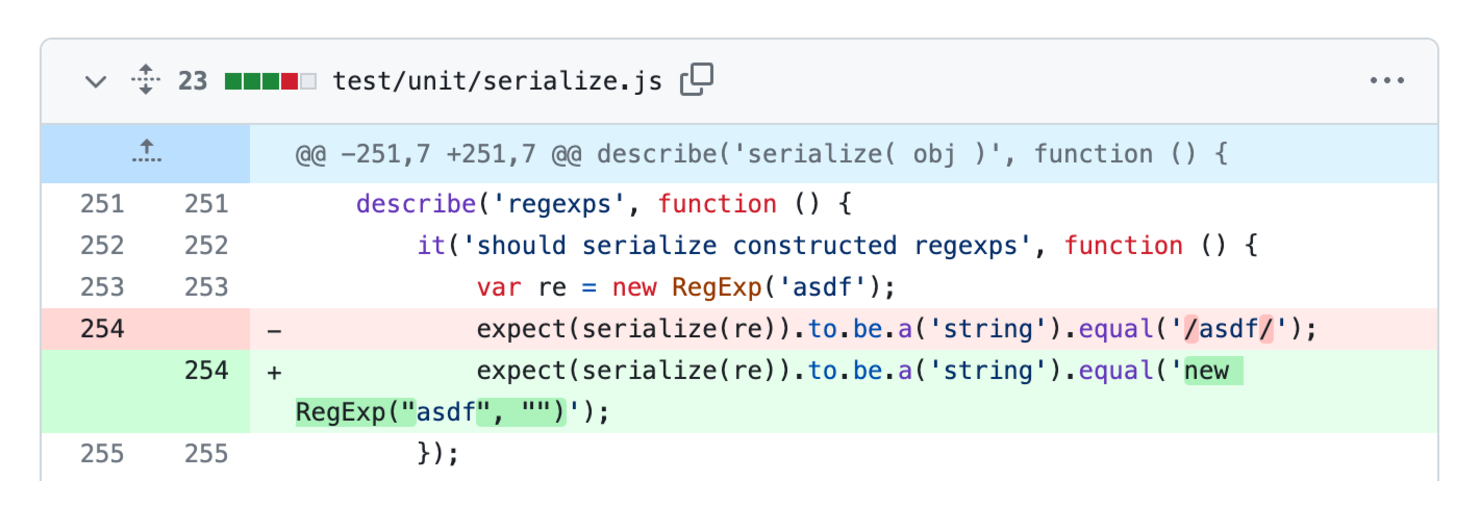
\includegraphics[width=1.0\linewidth]{fig/rq1/serialize-javascript/index.test.eps}
  \caption{serialize-javascriptのバージョン2.1.0から2.1.1への変更}
  \label{fig:motivation}
\end{figure}


クライアント開発者は,利用するライブラリのバージョンを更新する際に引き起こされるエラーを回避するために,更新後のバージョンの後方互換性を判断する必要がある.しかしながら関連研究が示すとおり,後方互換性を正確に判断することは多くの場合に困難である.

ライブラリの後方互換性は,ライブラリに付属するテストから判断できる場合がある.
テストへの変更内容から後方互換性を判断出来る例として,JavaScriptオブジェクトを文字列に変換する関数を提供するライブラリserialize-javascript\footnote{\url{https://github.com/yahoo/serialize-javascript/}}のバージョン2.1.0から2.1.1への更新を挙げる.
この更新ではセキュリティ修正のために,特定の入力に対する関数の出力が変更されている\footnote{\url{https://github.com/yahoo/serialize-javascript/compare/v2.1.0...v2.1.1}}.
実際の変更内容を図\ref{fig:sj}に示す.
図\ref{fig:motivation}上部の{\verb|index.js|}がソースコード,図下部の{\verb|test/unit/serialize.js|}がテストコードの変更内容である.
ソースコードの191行目で,190行目の条件に合致する特定の入力に対する関数の返り値が変更されている.この変更に伴って,対応するテストコードも修正されている.テストコードの254行目の変更では,テスト対象となる関数とパラメータはそのままで,期待する返り値のみ変更されている.後方互換性の損失に伴わないテストコード変更は,テストコードの実行手順の修正や,可読性向上のためのフォーマッティングなどが考えられる.ライブラリの後方互換性を判断する手段としてライブラリに付属しているテストへの変更を用いることができるが,多くの人気なライブラリに対してこの手法を適用した際に,どの程度の精度で後方互換性を判断できるのかは明らかになっていない.また,テストコードの変更内容には後方互換性の損失に伴う変更と伴わない変更がある.本研究ではこの仮説をもとに,継続的にテストが管理されているライブラリを対象として,ライブラリのテスト変更有無によって後方互換性を判断できるか否かを検証する.さらに,テストコードの変更内容をより詳細に分析することで,後方互換性の損失を正確に検出することを目指す.続く\ref{chap:rq1}章では,後方互換性の損失を含むライブラリ更新に伴うテストコードの変更内容を分析し,\ref{chap:rq2}章で後方互換性の損失に伴うテストコードの変更内容を自動検出するツールを開発し後方互換性の損失の検出精度を従来手法と比較検証する.



\section{分析手法}
\label{sec:analyticalMethod}

本章では\ref{sec:libraryVersioning}章の仮説を検証するために,ライブラリのテストに変更が加えられた場合に,変更後のライブラリがクライアントにとって破壊的変更を含むか否かを分析する.
本分析は2つの手順で構成する.
図\ref{fig:overview}は,分析手法の概略図を示す.

\begin{description}
\item[手順1] 破壊的変更を加えた可能性があるライブラリ更新の特定
\item[手順2] ライブラリ更新が破壊的変更を含むか否かを検証
\end{description}

本論文では,クライアントがライブラリの新しいバージョンを利用することで,クライアントテストが失敗した場合に,ライブラリの新しいバージョンに破壊的変更が加えられたと判断する.

\begin{figure}
  \centering
  \includegraphics[width=0.95\linewidth]{fig/overview.pdf}
  \caption{分析手法の概略図}
  \label{fig:overview}
\end{figure}

\subsection{手順1:破壊的変更を加えた可能性があるライブラリ更新の特定}
\label{sec:step1}
本分析では,ライブラリのバージョン更新に伴って,テストケースに変更が加えられた場合に,当該ライブラリを使用するクライアントに影響する破壊的変更を含む可能性があると考える.
手順1では,ライブラリのバージョン更新におけるテストケースの変更有無を分析する.
具体的には,分析対象とするライブラリからテストケースを収集し(\ref{sec:step1-1}項を参照),テストケースの変更内容に応じて破壊的変更を含む変更を加えた可能性のあるライブラリバージョンを特定する(\ref{sec:step1-2}項を参照).

\subsubsection{テストケースの収集}
\label{sec:step1-1}

分析対象とするライブラリの連続する2つのバージョンにおいて,古いバージョンを$L(X)$,新しいバージョンを$L(X+1)$とする.
\ref{sec:libraryVersioning}章で述べたようにライブラリの振る舞いがテストケースに反映されると考え,本分析では,ライブラリの変更に合わせてテストケースを変更することで,全てのテストを成功しているライブラリバージョンを対象とする.
$L(X+1)$においてテストが変更された場合は,開発者の要求変更などのために,破壊的変更を加えることが必要になったと考えられる.

バージョン$L(X)$と$L(X+1)$からそれぞれテストファイルを収集し,テストファイルからテストケースを抽出する.
このとき,テストケースの動作はテストケース以外のプログラムに依存している場合があるため,テストファイル中のテストケース以外のソースコードも同時に抽出する.
本研究ではJavaScript言語を対象とするため,JavaScript向けテストツールJest~\footnote{\url{https://jestjs.io/}}やMocha\footnote{\url{https://mochajs.org/}}で採用している慣習を基に,以下の規則でテストファイルの収集とテストケースの抽出を行う.

\begin{enumerate}
  \item \textbf{テストファイル収集} - ファイルパスに「test」または「spec」を含み,かつファイル名の末尾が{\verb|.js|}または{\verb|.ts|}であるファイルをテストファイルとして収集する.
  例えば,{\verb|test.js|}や{\verb|src/index.spec.js|}などをテストファイルと判断する.
  \item \textbf{テストケース抽出} - テストファイル内に記述されている,関数名がitまたはtestである関数呼び出しをテストケースとして抽出する.
  \item \textbf{テストケースに影響を与えるソースコード抽出} - 抽出したテストケースをテストファイルから削除し,残った文字列をテストケースに影響を与えるソースコードとして抽出する.
\end{enumerate}

Program~\ref{testSample}はテストファイルの例を示す.
抽出規則に従い,2行目から4行目のtest関数をテストケースとして抽出する.
その後,テストファイルからテストケースを除いて残った1行目がテストケースに影響を与えるソースコードとなる.

\begin{figure}[h]
    \begin{lstlisting}[caption={[upper/lower text]%
               \begin{tabular}[t]{@{}l@{}}
                test/sample.js \\[1.0\normalbaselineskip]
               \end{tabular}},frame={tb},numbers=left,label=testSample,identifierstyle={\small},xleftmargin=6mm]
const add = require("./add");
test("add arguments", function() {
    expect(add(1, 2)).toBe(3);
})
\end{lstlisting}
\end{figure}

\subsubsection{テストケースの変更の分類と後方互換性の判断}
\label{sec:step1-2}

本手法ではテストケースの変更を,従来研究と同様に4種類(追加,削除,修正,変更なし)に分類して,ライブラリバージョン間の後方互換性を判断する.
テストケースの変更内容を分類するために,テストケースとして抽出した関数について,第一引数をテストケースを一意に識別するラベル(Program~\ref{testSample}では,{\verb|"add arguments"|})とし,第二引数をテストケースの内容を示すボディ(Program~\ref{testSample}では,{\verb|function() { ... }|})とする.
テストケースのラベルとボディを用いて,$L(X)$から$L(X+1)$へのバージョン更新におけるテストケースの変更を4種類に分類する.

\begin{itemize}
\item \textbf{変更あり(追加)} $L(X)$のテストケースに存在しなかったラベルが,$L(X+1)$に存在する.
\item \textbf{変更あり(削除)} $L(X)$のテストケースに存在したラベルが,$L(X+1)$に存在しない.
\item \textbf{変更あり(修正)} $L(X)$のテストケースに存在したラベルが$L(X+1)$にも存在するが,ボディが異なる.
\item \textbf{変更なし} $L(X)$のテストケースに存在したラベルが$L(X+1)$にも存在し,ボディが同一である.
\end{itemize}

テストファイル中のテストケース以外の部分はテストケースに影響を与えるソースコードとして抽出する.
テストケースに影響を与えるソースコードの変更はライブラリの機能全体の振る舞いの変更と考え,テスト全体として\textbf{変更あり}と考える.

分類後,テストケースに\textbf{変更あり}が1つ以上含まれる,またはテストケースに影響を与えるソースコードが\textbf{変更あり}である場合,バージョン間に破壊的変更を含むと判断する.

\subsection{手順2:ライブラリ更新が破壊的変更を含むか否かを検証}
\label{sec:step2}

本分析では,ライブラリのバージョン更新に伴いライブラリに付属するテストに変更が加えられた場合に,当該ライブラリを使用する任意のクライアント$C$が有するテストが一つ以上失敗するか否かによって,ライブラリ更新が破壊的変更を含むか否かを検証する.

$C$の依存ライブラリの連続する2つのバージョン$L(X)$,$L(X+1)$をそれぞれ使用したときの$C$のテスト結果と,テスト結果に基づく破壊的変更の有無は,表\ref{fig:valid}に示す4つに分類される.

\begin{table}[h]
  \centering
  \caption{$C$が$L(X)$または$L(X+1)$を使用した時のテスト結果に基づく破壊的変更の有無}
  \label{fig:valid}
  \scalebox{0.8}{
  \begin{tabular}{p{2.3cm}|p{2.6cm}|p{2cm}}\hline
    $L(X)$を使用した$C$のテスト結果 & $L(X+1)$を使用した$C$のテスト結果 & 破壊的変更 \\ \hline
    成功 & 失敗 & あり \\ \hline
    成功 & 成功 & 不明 \\ \hline
    失敗 & 失敗 & 不明 \\ \hline
    失敗 & 成功 & 不明 \\ \hline
  \end{tabular}
  }
\end{table}

$L(X)$を使用した$C$のテストが成功し,$L(X+1)$を使用した$C$のテストが失敗した場合,ライブラリの変更のみによって$C$のエラーが引き起こされたと判断でき,$L(X)$から$L(X+1)$へのライブラリ更新には破壊的変更が含まれると分かる.
一方で,$L(X)$と$L(X+1)$の両方で$C$のテストが成功する場合であっても,ライブラリの変更に破壊的変更が含まれないとは限らない.
なお,$L(X)$を使用した$C$のテストが失敗した場合,破壊的変更有無は不明となるため分析しない.

以上の手順1と手順2を分析対象とするライブラリのバージョン更新に適用し,結果を図~\ref{fig:overview}中の混同行列の4つに分類する.

\section{分析準備}
\label{sec:prepare}

分析対象とするライブラリバージョンと,後方互換性を判断するためのクライアントテストの実行結果を収集する.

\subsection{分析対象ライブラリの決定}
本分析ではMujahidらのデータセット\cite{Dataset}を使用する.
データセットには,GitHubリポジトリが記載されていることと,依存ライブラリを記述するファイル({\verb|package.json|})の変更履歴が2回以上あることを条件に,npmから収集した290,417件のJavaScriptライブラリが含まれている.
本研究ではこのデータセットから,3つの条件を満たすライブラリを使用する.

\begin{itemize}
\item テストが付属していること.ライブラリがテストケースに加えた変更を利用して後方互換性を判断する(\ref{sec:step1}項を参照)ため.
\item ライブラリの人気度合いを示すnpmスコア~\footnote{\url{https://npms.io/}}が上位500件以内であること.人気なライブラリを対象とするため.
\item 各バージョンがリリースされた変更のコミットステータス\footnote{\url{https://docs.github.com/en/rest/reference/repos#statuses}}からテスト実行結果を確認し,テスト実行時の成功率が100\%であること.テストを継続的に管理しているライブラリを対象とするため.
\end{itemize}

ライブラリが持つGitHubリポジトリの各変更には,コミットステータスと呼ばれる,テストの実行結果を含むデータが紐付けられている.
例として,serialize-javascriptは変更履歴\footnote{\url{https://github.com/yahoo/serialize-javascript/commits/2b4f837}}に登録されているコミットステータスを確認できる.%図\ref{fig:commitStatus}に示す.
serialize-javascriptの2022年1月19日の変更では,依存ライブラリのバージョンが変更されている.
この変更が行われた際に,同時にテストが実行され,実行結果がコミットステータスに登録されている.
登録されている情報からテストはいずれも成功していると分かる.
コミットステータスを使用することで,分析のためにテストを再度実行することなく,既存のテスト実行結果を利用する.

%\begin{figure}
%  \centering
%  \includegraphics[width=0.95\linewidth]{fig/commit-status.png}
%  \caption{serialize-javascriptのGitHubリポジトリに登録されているコミットステータス}
%  \label{fig:commitStatus}
%\end{figure}

上記の条件を満たす238件のライブラリを分析対象とする.

\subsection{分析対象ライブラリの各バージョンごとにクライアントテスト実行結果を収集}
\label{sec:experiment}
ライブラリバージョンの後方互換性を判断した後,後方互換性を検証するためにクライアントテスト実行結果を利用する(\ref{sec:step2}項を参照)ため,分析対象ライブラリの各バージョンごとにクライアントテスト実行結果を収集する.

分析対象とする238件のライブラリと,各ライブラリのいずれかのバージョンに依存するクライアントとの組み合わせをMujahidらのデータセットから抽出した.
抽出結果について,各ライブラリごとのクライアント数を図\ref{fig:dependencies}に示す.
横軸はクライアント数ごとに並べ替えた各ライブラリ,縦軸は各ライブラリのクライアント数を示す.
238件のライブラリには平均93.6件,中央値36件のクライアントがあり,ライブラリバージョンとクライアントの組み合わせは22,271組を確認した.

各ライブラリバージョンとクライアントの組について,2つの手順を繰り返すことでクライアントテスト実行結果を収集する.

\begin{enumerate}
  \item クライアントテストを実行する.テストが失敗した場合は手順を終了する.
  \item ライブラリのバージョンを一つ新しいものに更新し,1.に戻る.新しいバージョンが無ければ手順を終了する.
\end{enumerate}

あるクライアント$C$とライブラリ$L$のバージョン$X$との組を使用し,手順を繰り返す例を図\ref{fig:experimentExample}に示す.
例では,手順1と手順2を2回繰り返した後,手順1におけるクライアントテスト実行が失敗することで終了し,最終的にクライアントテスト結果を3件収集する.
3件のテスト結果において,$L(X+1)$を使用して成功した$C$のテストが$L(X+2)$使用時に失敗していることから,テスト結果を変化させる破壊的な変更がライブラリに含まれていることがわかる.
一方で,$L(X)$を使用して成功していた$C$のテストは,$L(X+2)$使用時にも成功しているため,$L(X+1)$の後方互換性は不明である.

\begin{figure}
  \centering
  \includegraphics[width=0.6\linewidth]{fig/dependencies.pdf}
  \caption{分析対象ライブラリ(238件)ごとのクライアント数の分布(1≦n≦238)}
  \label{fig:dependencies}
\end{figure}

\begin{figure}
  \centering
  \includegraphics[width=0.5\linewidth]{fig/experiment-example.pdf}
  \caption{クライアントテスト実行結果収集の例}
  \label{fig:experimentExample}
\end{figure}

クライアントテストが失敗したライブラリバージョンに以降のバージョンについては,再度クライアントテストが成功することは見込めないため分析しない.
上記手順によって71,342件のクライアントテストを実行し,結果を収集した.

\subsection{テスト結果に基づいて分析対象ライブラリバージョンを決定}
\ref{sec:experiment}項で収集した結果に基づいて,後方互換性を判断するライブラリバージョンを決定し,後方互換性を検証するための各クライアントテストの結果を3つの手順で集計する.

\begin{enumerate}
  \item \ref{sec:experiment}項で,最終的にテスト結果を1件しか収集できず,$L(X)$と$L(X+1)$の組ができないものを除く.
  \item 全てのクライアントテスト結果について,$L(X)$と$L(X+1)$,$L(X+1)$と$L(X+2)$のようにバージョン更新ごとの組を作る.
  \item 異なるクライアントが同じライブラリバージョンの組を使用した場合はクライアントテスト実行結果を統合する.
\end{enumerate}

集計の結果,2,111組の分析対象ライブラリバージョンを決定した.

\section{分析結果}
\label{sec:result}

分析準備で収集したデータセットに対して\ref{sec:analyticalMethod}章で述べた分析手法を適用した.
結果を表\ref{fig:result}に示す.
分析対象とするライブラリバージョン2,111件中,テストケースの変更を含む(破壊的変更を加えた可能性が高い)ライブラリバージョンは1,039件(約49\%),変更を含まない(破壊的変更を加えた可能性が低い)ライブラリバージョンは1,072件(約51\%)であった.

破壊的変更を加えた可能性が高いライブラリバージョン1,039件中183件(約18\%)は1件以上のクライアントテストが失敗し,1,039件中856件(約82\%)のライブラリバージョンを使用するクライアントテストは成功していた.
クライアント数が不足している場合はライブラリのテストケースの変更可否のみで後方互換性の有無を検出できないと考えられる.
また,分析対象としたライブラリバージョンのうち,クライアントテストが1件以上失敗した268件を確認し,バージョン更新後のライブラリにテストケースの変更を含むか否かだけで,183件(約68\%)の破壊的変更を加えたライブラリバージョンを特定した.
残り85件(約32\%)はライブラリ更新時のテスト変更漏れなどが考えられる.
実際にテストを調査した内容については,\ref{sec:discussion}章で言及する.

\begin{table}[h]
  \centering
  \caption{分析結果}
  \label{fig:result}
  \scalebox{0.8}{
  \begin{tabular}{p{2.8cm}|p{1.7cm}|p{1.7cm}|p{1cm}}\hline
     & テスト変更あり & テスト変更なし & 合計 \\ \hline
    クライアントテストが一つ以上失敗 & 183 & 85 & 268 \\ \hline
    クライアントテストが全て成功 & 856 & 987 & 1,843 \\ \hline
    合計 & 1,039 & 1,072 & 2,111 \\ \hline
  \end{tabular}
  }
\end{table}


\section{分析結果}\label{seq:rq1-result}

\begin{figure}[t]
  \centering
  \includegraphics[width=1.0\linewidth]{fig/barh-test-pattern.pdf}
  \caption{テスト変更内容ごとの実際の後方互換性}
  \label{fig:test_pattern}
\end{figure}

図\ref{fig:test_pattern}は,テスト変更内容ごとの後方互換性の有無を横棒積み上げ棒グラフで示す.横軸は各テストコード変更の発生件数,縦軸は各テストコード変更内容である.破線より上は,従来手法で後方互換性を維持すると判定するテスト変更内容であり,破線より下は従来手法で後方互換性を損失すると判定するテスト変更内容である.

\subsection{従来手法で後方互換性を維持すると判定するテスト変更内容}
従来手法で後方互換性を維持すると判定するテスト変更内容は,テストスイートの追加,テストケースの追加である.これらは,後方互換性を維持するライブラリ更新に伴う場合が多いため,従来手法で誤検出となる主な原因ではない.ただし,後方互換性を損失するライブラリ更新に伴ってテストスイートやテストケースを追加する場合もある.具体的な例は\ref{subsec:add-test}項で述べる.

\subsection{従来手法で後方互換性を損失すると判定するテスト変更内容}
従来手法で後方互換性を損失すると判定するテスト変更内容は,テストスイートの削除,テストケースの削除,アサーションの追加,アサーションの削除,アサーションの入力値の変更,アサーションの期待値の変更,前提条件の変更,テストフィクスチャの変更,リファクタリングである.このうち,リファクタリングは後方互換性を維持するライブラリ更新に伴う場合が多く,件数も多いため従来手法で誤検出となる主な原因であるとわかる.一方,リファクタリングが後方互換性を損失するライブラリ更新に伴う場合もある.これは,後方互換性を損失するライブラリ更新に伴って,無関係にテストがリファクタリングされることがあることを示す.テストスイートの削除,テストケースの削除は,後方互換性を損失するライブラリ更新に伴う場合が多いため,従来手法で誤検出となる主な原因ではない.ただし,後方互換性を維持するライブラリ更新に伴ってテストスイートやテストケースを削除する場合もある.具体的な例は\ref{subsec:delete-test}項で述べる.アサーションの追加,アサーションの入力値の変更,アサーションの期待値の変更,前提条件の変更は,後方互換性を維持するライブラリ更新に伴う場合が多く,従来手法で誤検出となる主な原因である.ただし,後方互換性を損失するライブラリ更新に伴って,アサーションを追加したり,アサーションの入力値,アサーションの期待値を変更する場合もある.具体的な例は,それぞれ\ref{subsec:add-test}項,\ref{subsec:change-test}項で述べる.テストフィクスチャの変更は,テストデータの初期化や事前条件を定義する性質上,変更時のテストコードの影響範囲が広く,後方互換性の損失との関係を分析することが困難であるため,本研究では対象としない.

続く\ref{rq2:kousatu}節では,テスト変更内容をテストコード追加,テストコード削除,テストコード変更に分けて,後方互換性を損失するライブラリ更新に伴うテストコード変更内容,伴わないテストコード変更内容をそれぞれ例を挙げて考察し,後方互換性の損失を検出する手掛かりとなるテストコード変更内容を特定する.

\section{考察}\label{sec:rq1.kousatu}

\subsection{テストコード追加}\label{subsec:add-test}

\begin{figure}[t]
  \centering
  \includegraphics[width=1.0\linewidth]{fig/rq1/set-map/map.pdf}
  \caption{serialize-javascriptのバージョン1.6.1から1.7.0のソースコード変更差分}
  \label{fig:rq1.insert-test-src}
\end{figure}

\begin{figure}[t]
  \centering
  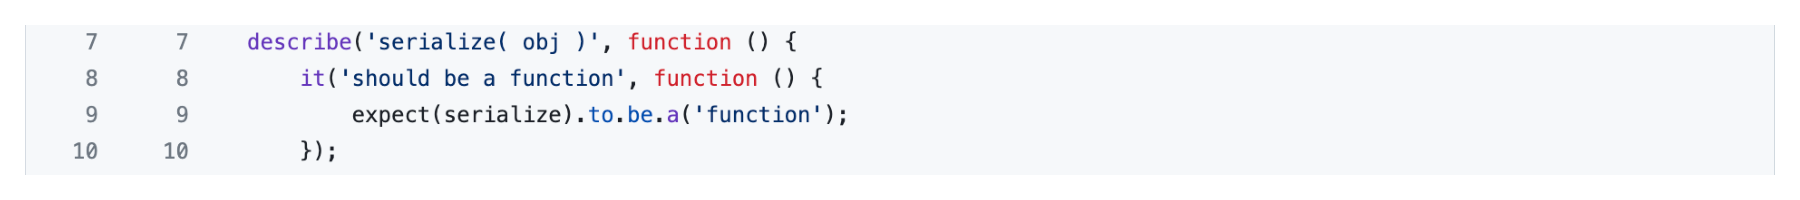
\includegraphics[width=1.0\linewidth]{fig/rq1/set-map/map.test.1.eps}
  \includegraphics[width=1.0\linewidth]{fig/rq1/set-map/map.test.2.eps}
  \caption{serialize-javascriptのバージョン1.6.1から1.7.0のテストコード変更差分}
  \label{fig:rq1.insert-test-test}
\end{figure}

テストコード追加は,テスト対象となるAPIの追加など後方互換性を維持するライブラリ更新に伴う場合が多い.ただし,後方互換性を損失するライブラリ更新に伴ってテストコードが追加されることがある.例として,JavaScriptオブジェクトを文字列に変換するAPIを提供するライブラリserialize-javascriptのバージョン1.6.1から1.7.0へのマイナーアップデート\footnote{\url{https://github.com/yahoo/serialize- javascript/compare/v1.6.1...v1.7.0}}を挙げる.図\ref{fig:rq1.insert-test-src}はソースコードの変更差分,図\ref{fig:rq1.insert-test-test}はテストコードの変更差分を示す.この変更では,関数{\verb|serialize|}に,JavaScriptの{\verb|Map|}型のデータを文字列に変換する機能が追加された(図\ref{fig:rq1.insert-test-src},155行目から157行目).この変更に伴って,関数{\verb|serialize|}に関するテストスイート(図\ref{fig:rq1.insert-test-test},7行目)に,新しく{\verb|Map|}型のデータが正確に文字列に変換されるかを検証するテストスイートが追加された(図\ref{fig:rq1.insert-test-test},201行目から220行目).バージョン1.6.1では,関数{\verb|serialize|}は{\verb|Map|}型の入力を文字列に変換する機能を持っていないため,文字列に変換されないことに依存しているクライアントはバージョン更新の際に返り値が新しくなったことによる影響を受ける.このようなAPIの機能拡張による後方互換性の損失は,図\ref{fig:rq1.insert-test-test}で示すように既存のテストスイート内にテストコードが追加されるという特徴があるため,既存のテストスイート内にテストスイート,テストケース,アサーションが追加された場合,ライブラリの後方互換性が損失したと判断できると考えられる.

\subsection{テストコード削除}\label{subsec:delete-test}

\begin{figure}[t]
  \centering
  \includegraphics[width=1.0\linewidth]{fig/rq1/uuid/randomBytes2.pdf}
  \includegraphics[width=1.0\linewidth]{fig/rq1/uuid/randomByte.pdf}
  \caption{uid-safeのバージョン2.0.0から2.1.0のソースコード変更差分}
  \label{fig:rq1.delete-test-src}
\end{figure}

\begin{figure}[t]
  \centering
  \includegraphics[width=1.0\linewidth]{fig/rq1/uuid/randomByte-test.pdf}
  \caption{uid-safeのバージョン2.0.0から2.1.0のテストコード変更差分}
  \label{fig:rq1.delete-test-test}
\end{figure}

テストコード削除は,テスト対象となるAPIの削除など後方互換性を損失するライブラリ更新に伴う場合が多い.ただし,後方互換性を維持するライブラリ更新に伴ってテストコードが削除されることがある.例として,暗号化されたUIDを生成するAPIを提供するライブラリuid-safeのバージョン2.0.0から2.1.0へのマイナーアップデート\footnote{\url{https://github.com/crypto-utils/uid-safe/compare/2.0.0...2.1.0}}を挙げる.図\ref{fig:rq1.delete-test-src}はソースコードの変更差分,図\ref{fig:rq1.delete-test-test}はテストコードの変更差分を示す.この変更では,セキュリティ上の問題から,ランダムなバイト列を生成する関数{\verb|randomBytes|}を削除(図\ref{fig:rq1.delete-test-src},99行目から107行目)し,同等のモジュールに置き換えている(図\ref{fig:rq1.delete-test-src},16行目).この変更に伴って,関数{\verb|randomBytes|}の動作を検証するテストスイートが削除されている(図\ref{fig:rq1.delete-test-test},40行目から54行目).モジュールの置き換え前後で関数{\verb|randomBytes|}の振る舞いが全く同じ場合,後方互換性が維持される.本研究では,\ref{subsec:kouhougokanseinohantei}章で述べた通り,後方互換性の有無の判定にクライアントテストを利用している.このようなモジュールに置き換える例では,振る舞いの変化が限定的になるため,クライアントテストが捉えられず後方互換性を維持したと誤判定されることが考えられる.誤判定を防ぐには実際に影響を受けるクライアントの特定が必要になるが,容易ではない\cite{detecting-locations-in-js}.本研究では,件数も少なく結果への影響が少ないと考えられるため今後の課題とする.

\subsection{テストコード変更}\label{subsec:change-test}

\begin{figure}[t]
  \centering
  \includegraphics[width=1.0\linewidth]{fig/rq1/rejection/rejection-test.pdf}
  \caption{loud-regectionのバージョン1.2.1から1.3.0のテストコード変更差分}
  \label{fig:rq1.change-test-rejection-test}
\end{figure}

\begin{figure}[t]
  \centering
  \includegraphics[width=1.0\linewidth]{fig/rq1/rgb/rgb-src.pdf}
  \includegraphics[width=1.0\linewidth]{fig/rq1/rgb/rgb-src-1.pdf}
  \caption{color-stringのバージョン0.4.0から1.0.0のソースコード変更差分}
  \label{fig:rq1.change-test-input-src}
\end{figure}

\begin{figure}[t]
  \centering
  \includegraphics[width=1.0\linewidth]{fig/rq1/rgb/rgb-test.pdf}
  \caption{color-stringのバージョン0.4.0から1.0.0のテストコード変更差分}
  \label{fig:rq1.change-test-input-test}
\end{figure}

アサーションの入力値,期待値の変更やリファクタリングなどのテストコード変更は,ライブラリの更新とは無関係に行われることが多い.ライブラリの更新とは無関係にアサーションの入力値,期待値が変更される例として,非同期処理のエラー内容を追跡するAPIを提供するライブラリloud-regectionのバージョン1.2.1から1.3.0へのマイナーアップデート\footnote{\url{https://github.com/sindresorhus/loud-rejection/compare/v1.2.1...v1.3.0}}を挙げる.図\ref{fig:rq1.change-test-rejection-test}はテストコードの変更差分を示す.この変更では,アサーションメソッドを{\verb|true()|}から{\verb|regex()|}に変更しており,アサーションの入力値と期待値が同時に変更されている.ただし,テストコードの振る舞いは変わっておらず,ソースコードの変更とは無関係のテストコード変更である.一方,後方互換性を損失するライブラリ更新に伴って,アサーションの入力値,期待値が変更されることがある.アサーションの期待値が変更される例は,\ref{sec:key-idea}節で示したので割愛する.後方互換性を損失するライブラリ更新に伴ってアサーションの入力値が変更される例として,CSSの色文字列を解析するAPIを提供するライブラリcolor-stringのバージョン0.4.0から1.0.0のメジャーアップデート\footnote{\url{https://github.com/Qix-/color-string/compare/0.4.0...1.0.0}}を挙げる.図\ref{fig:rq1.change-test-input-src}はソースコードの変更差分,図\ref{fig:rq1.change-test-input-test}はテストコードの変更差分を示す.この変更では,関数{\verb|rgbString|}を{\verb|to.rgb|}に置き換えている(図\ref{fig:rq1.change-test-input-src},154行目から160行目,129行目から135行目).この変更に伴って,関数{\verb|rgbString|}に関するアサーションの入力値が変更されている.図\ref{fig:rq1.change-test-input-test}の62行目から68行目と68行目から74行目は1行ずつ対応しており,アサーションの{\verb|equal|}関数の第一引数の入力値が変更され,第二引数の期待値は変更されていない.以上から,APIの入出力形式の変更による後方互換性の損失は,アサーションの期待値もしくは入力値のいずれか一方だけ変更されるという特徴があるため,アサーションの入力値と期待値のいずれか一方が変更された場合,後方互換性を損失したと判断できると考えられる.


\section{まとめ}
本章では,後方互換性を損失するライブラリ更新に伴ってどのようなテストコード変更が行われているかを分析し,後方互換性の損失を検出する手掛かりとなるテストコード変更内容を明らかにした.結果「既存のテストスイート内でのテストコード追加」「テストコード削除」「アサーションの入力値と期待値のいずれか一方の変更」の3つが後方互換性の損失を検出する手掛かりになる,機械的に検出可能なテストコード変更であると考える.

\section{RQ2:テストコード変更内容に基づく後方互換性損失の検出手法の有効性はどの程度か?}\label{chap:rq2}

\section{概要}
本章では,\ref{chap:rq1}章で述べた,後方互換性を損失するライブラリ変更に伴うテストコード変更内容である「既存のテストスイート内でのテストコード追加」「テストコード削除」「アサーションの入力値と期待値のいずれか一方の変更」を自動検出するツールを開発し,後方互換性の損失の検出精度を従来手法と比較検証する.まず,変更前後のソースファイルからプログラムの変更箇所と,その変更箇所の変更方法(追加・削除など)を分類する.その後,変更箇所とその変更方法が条件に一致すれば後方互換性を損失したと判定する.

\section{提案手法}\label{sec:rq2.teian}

本研究が提案する自動検出ツールは,入力を全てのソースファイル,出力を後方互換性の有無の予測とする.まず,入力として与えられた変更前後の全てのソースファイルから,変更されていないファイルを除外し,テストコードが記述されたファイルを抽出する.従来研究\cite{matsuda}では,テストコードが記述されたファイルの条件を,ファイルパスに{\verb|test|}または{\verb|spec|}を含み,ファイル名の末尾が{\verb|.js|}または{\verb|.ts|}であるファイルとする.本研究ではこの条件に加え,ファイル名の末尾が{\verb|.d.ts|}でないファイルを条件とする.ファイル名の末尾が{\verb|.d.ts|}であるファイルは型定義ファイルであり本研究では除外する.次に,抽出したソースファイルにおける,プログラムの変更箇所とその変更方法を\ref{subsec:rq2.astseisei}項の方法で特定する.最後に,プログラムの変更箇所とその変更方法が\ref{subsec:rq2.jouken}項で述べる3つの条件に1つでも一致すれば,後方互換性が損失していると判定し,いずれにも一致しなければ後方互換性を維持していると判定する.

\subsection{プログラムの変更箇所と変更方法の特定}\label{subsec:rq2.astseisei}
プログラムの変更箇所と変更方法の特定のために,差分解析ツールであるGumTree\cite{gumtree}を使用する.GumTreeは,ソースコードの構造を表す木構造データ(抽象構文木)を基にした差分解析ツールである.構造単位で比較するため,行単位の差分解析に比べて細かい変更箇所の特定が可能になる.また,他の抽象構文木(以降,AST)を基にした差分解析ツール\cite{diff-1}\cite{diff-2}\cite{diff-3}と比べて精度が高く,JavaやJavaScriptなど複数のプログラミング言語に対応している.GumTreeは,変更前後のソースファイルまたはASTを受け取ると,それらを比較してASTのノード単位の編集操作を出力する.検出できる編集操作は,「削除」「挿入」「移動」「変更」である.ただし,GumTreeはファイル単位の差分しか検出することができず,ファイルを横断するソースコードの移動操作に対して「移動」ではなく「削除と挿入」として出力されてしまう.ファイルを横断するテストコードの移動はリファクタリングにおいて一般的に行われるため誤検出の原因となる.本手法では,藤本らの手法\cite{gumtreenoyatu}を一部利用し,次の手順で複数ファイルを横断してGumTreeを適用する.

\begin{enumerate}
  \setlength{\itemsep}{0cm}
  \item 変更のある各ファイルごとにASTを生成する
  \item 根となるノードを1つ作成する
  \item 各ファイルごとに生成したASTを子ノードとして加えていく
  \item 1から3を変更前後で実施し,2つASTを生成する
  \item 変更前後で生成された2つのASTをGumTreeに入力して出力を得る
\end{enumerate}

この方法により,バージョン間のテストコード変更に対して,プログラムの変更箇所(ノード)と,「削除」「挿入」「移動」「変更」の4つの変更方法をファイルを横断する移動操作も含めて特定することができる.

\subsection{後方互換性を損失したバージョンの判定条件}\label{subsec:rq2.jouken}
\ref{chap:rq1}章で述べた,「既存のテストスイート内でのテストコード追加」「テストコード削除」「アサーションの入力値と期待値のいずれか一方の変更」を自動で検出するために,それぞれ条件を定義する.

まず,「既存のテストスイート内でのテストコード追加」「テストコード削除」を判定するために,テストコードを定義する.従来研究\cite{matsuda}では,テストファイル内に記述されている,関数名が{\verb|it|}または{\verb|test|}である関数呼び出しをテストケースとしている.本研究では,テストスイートの追加・削除を含めるため,慣習的にテストスイートの宣言として使われる関数名{\verb|describe|}を加え,{\verb|it|}または{\verb|test|}または{\verb|describe|}のいずれかの関数呼び出しで,第一引数が文字列,第二引数が関数であるものをテストスイートまたはテストケースと定義する.

次に,「アサーションの入力値と期待値のいずれか一方の変更」を判定するために,アサーションの入力値と期待値を定義する.JavaScript言語では,アサーションの書き方はフレームワークによって異なる.本手法では,State of JavaScript 2022\footnote{\url{https://2022.stateofjs.com/}}で紹介されている主要なテストフレームワーク13件のうち,単体テストで使われるフレームワーク5件(Jest\footnote{\url{https://jestjs.io/}},Mocha\footnote{\url{https://mochajs.org/}},AVA\footnote{\url{https://github.com/avajs/ava}},Jasmine\footnote{\url{https://jasmine.github.io/}},Vitest\footnote{\url{https://vitest.dev/}})を対象とする.Mochaは複数のアサーションの記述スタイルを利用できるため,Mochaで使用可能なアサーションのスタイルについても対象とする.テストフレームワーク毎のアサーションの書き方は,大きく2つに大別できる.例をProgram\ref{bdd.test.js},Program\ref{tdd.test.js}で示す.

\begin{lstlisting}[caption=アサーション例1, label=bdd.test.js]
expect(calculator.add(1, 1)).to.be.a('number').equal(2);
expect(calculator.add(1, 1), 'to be', 2);
calculator.add(1, 1).should.be.a('number').equal(2);
\end{lstlisting}

Program\ref{bdd.test.js}は,自然言語に似た構文を使用してテストを記述する記述形式で,Jest,Mocha,Jasmine,Vitestで使用される.その中でも,1行目のように,{\verb|expect|}関数にメソッドチェーンで振る舞いを記述する形式,2行目のように{\verb|expect|}関数の引数にそのまま振る舞いを記述する形式,3行目のように入力値に{\verb|should|}プロパティを追加して振る舞いを記述する形式がある.1,2行目の形式に対しては,{\verb|expect|}関数の第一引数を入力値,それ以降を期待値として扱い,3行目の形式に対しては,{\verb|should|}プロパティ以前を入力値,以降を期待値として扱う.

\begin{lstlisting}[caption=アサーション例2, label=tdd.test.js]
assert.equal(calculator.add(1, 1), 2);
t.is(calculator.add(1, 1), 2);  
t.true(calculator.add(1, 1) === 2);
\end{lstlisting}

Program\ref{tdd.test.js}は,Node.js\footnote{\url{https://nodejs.org/en}}標準の{\verb|assert|}文がメインの記述形式で,AVA,Mochaで使用される.その中でも,1行目や2行目のように,第一引数に入力値,第二引数に期待値を取る形式と,3行目のように入力だけを引数に取る形式がある.この記述形式に対しては,{\verb|assert|},{\verb|t|},{\verb|test|}をキーとして,アサーションメソッドの第一引数を入力,第二引数を期待値として扱う.3行目のように引数が1つの場合は,引数を入力,アサーションメソッド名を期待値とする.

これらのテストコードの定義を利用し,後方互換性を損失するライブラリ更新に伴うテストコード変更内容である,「既存のテストスイート内でのテストコード追加」「テストコード削除」「アサーションの入力値と期待値のいずれか一方の変更」を検出する3つの条件を定める.

\begin{description}
  \item[\textbf{既存のテストスイート内でのテストコード追加}]:GumTreeで「挿入」と判定された変更箇所がテストコードまたはアサーションであり,かつ既存のテストコード内で追加されていること
  \item[\textbf{テストコード削除}]:GumTreeで「削除」と判定された変更箇所がテストコードであること
  \item[\textbf{アサーションの入力値と期待値のいずれか一方の変更}]:GumTreeで「変更」と判定された変更箇所がアサーションの入力値もしくは期待値であり,同一アサーションの入力値もしくは期待値がGumTreeで「変更」と判定されていないこと
\end{description}

ライブラリバージョンに含まれるテストコード変更内容が,以上3つの条件に1つでも当てはまれば,ライブラリバージョンは後方互換性を損失したと判定し,1つも当てはまらなければライブラリバージョンは後方互換性を維持したと判定する.

\section{データセット}
データセットは,\ref{rq1:datasets}節と同様の従来研究\cite{matsuda}で収集されたライブラリバージョン2,111件を使用し,削除や非公開になったことによりGitHub上でアクセスできないものと,GumTree上でエラーになるもの計156件を除いた1,955件を使用する.

\section{分析結果}

\begin{table}[t]
\centering
\caption{提案手法と従来手法の比較結果}
\label{fig:result}
\begin{tabular}{cl|r|r|r}
\hline
\multicolumn{2}{c|}{} & \multicolumn{1}{c|}{後方互換性なし} & \multicolumn{1}{c|}{後方互換性あり} & \multicolumn{1}{c}{合計} \\ \hline
\multicolumn{1}{c|}{\multirow{3}{*}{提\newline 案\newline 手\newline 法}} & 後方互換性なしと判定      & 114 & 548 & 662 \\ \cline{2-5} 
\multicolumn{1}{c|}{}                                                      & 後方互換性ありと判定      & 109 & 1,184 & 1,293 \\ \cline{2-5} 
\multicolumn{1}{c|}{}                                                      & 合計              & 223 & 1,732 & 1,955 \\ \hline
\multicolumn{1}{c|}{\multirow{3}{*}{従\newline 来\newline 手\newline 法}} & 従来手法で後方互換性なしと判定 & 140 & 765 & 905 \\ \cline{2-5} 
\multicolumn{1}{c|}{}                                                      & 従来手法で後方互換性ありと判定 & 83  & 967 & 1,050 \\ \cline{2-5} 
\multicolumn{1}{c|}{}                                                      & 合計              & 223 & 1,732 & 1,955 \\ \hline
\end{tabular}
\end{table}

データセットに対して,従来手法と\ref{sec:rq2.teian}節で述べた手法を適用した結果を表\ref{fig:result}に示す.分析対象とするライブラリバージョン1,955件中,提案手法で後方互換性なしと判定したライブラリバージョンは662件(約34%),後方互換性ありと予測したライブラリバージョンは1,293件(約66%)であった.また,従来手法で後方互換性なしと予測したライブラリバージョンは905件(約46%),後方互換性ありと予測したライブラリバージョンは1,050件(54%)であった.

提案手法で後方互換性を損失したと判定したライブラリバージョン662件中,114件(約17%)は後方互換性を損失し(適合率),662件中548件(約83%)は後方互換性を維持している.また,後方互換性を損失したライブラリバージョン223件中,114件(約51%)を正しく予測した(再現率).従来手法では,後方互換性を損失したと予測したライブラリバージョン905件中,140件(約15%)が後方互換性を損失(適合率)し,後方互換性を損失したライブラリバージョン223件中,140件(63%)を正しく予測した(再現率).

従来手法では,後方互換性を維持するライブラリバージョンに対し,後方互換性を損失したと誤検出した件数は765件であり,提案手法は548件が誤検出であった.これは,従来手法で誤検出となる,テストケースの移動やラベルの修正などのテストコードのリファクタリングによる影響を提案手法では受けないため,誤検出を減らすことができたことを示している.一方で,提案手法は従来手法に比べて,後方互換性を損失したライブラリバージョンの検出精度が低下している.従来手法では後方互換性を損失したライブラリバージョン223件中,140件を正確に検出できたのに対し.提案手法では114件のみを検出した.この結果から,提案手法は誤検出を減らすことには成功しているが,後方互換性を損失したライブラリバージョンの検出においては改善の余地があるとわかる.予測結果を目視により調査した内容については,\ref{rq2:kousatu}章で言及する.

\section{考察}
\label{sec:discussion}
分析したライブラリバージョンを手動で確認し,確認したライブラリバージョンの例をあげて分析結果の適合率と再現率について考察する.
また,本研究の妥当性への脅威を述べる.

\subsection{適合率:テスト変更を含むライブラリバージョンにおける破壊的変更}
破壊的変更を加えた可能性が高いと判断した1,039件のライブラリバージョンのうち,856件は全てのクライアントテストが成功しているため,実際の後方互換性は判断できない.
テストケースの削除や修正が行われたが,それに伴って影響を受けるクライアントが存在しなかった原因を考察する.
まず,ライブラリバージョンの後方互換性が維持されていたため,全てのクライアントに影響を与えなかったことが考えられる.
例として,値がStreamオブジェクトであることを検証する関数を提供するライブラリであるis-streamのバージョン1.0.1から1.1.0への変更~\footnote{\url{https://github.com/sindresorhus/is-stream/compare/v1.0.1...v1.1.0}}を図\ref{fig:isStream}に示す.
この変更ではライブラリに新しいAPIが追加されており,既存のクライアントに影響を与えない.
is-streamへの変更は破壊的変更ではないが,変更と同時にテストを実行するツールのバージョンも更新され,更新に伴ってテストケースが変更されている.
テストケースが変更されているため,本分析ではis-streamのバージョン1.1.0は後方互換性を損失していると誤って判断した.
テストの誤り修正や実行手順の変更など,ライブラリの変更とは無関係にテストにも変更が加えられることがあるため,テストの変更内容についても分類を行うことでさらに精度が向上すると期待できる.

\begin{figure}
  \vspace{1zh}
  \centering
  \includegraphics[width=0.95\linewidth]{fig/is-stream.png}
  \caption{is-streamのバージョン1.0.1から1.1.0におけるライブラリの変更}
  \label{fig:isStream}
\end{figure}

次に,後方互換性を損失しているが,クライアントテストが実行するライブラリの機能が限定的であったためにその影響が確認できなかったことが考えられる.
例として,値が絶対URLであることを検証するライブラリであるis-absolute-urlのバージョン3.0.0から3.0.1への変更~\footnote{\url{https://github.com/sindresorhus/is-absolute-url/compare/v3.0.0...v3.0.1}}を図\ref{fig:isAbsoluteUrl}に示す.
この変更では入力としてURLではなくWindows形式のファイルパスが与えられた場合に{\verb|false|}を返すよう関数が変更されている.
is-absolute-urlへの変更は特定の入力に対する結果が変化したという点で破壊的な変更であるが,本分析でis-absolute-urlのバージョン3.0.1を使用してテストを実行したクライアントは4件しかなかったため,破壊的変更の影響が現れなかったと考えられる.
破壊的変更が行われた機能をクライアントが利用していなかった場合,後方互換性の損失は確認できない.
クライアント数が不足しているライブラリを除外した場合の結果については\ref{sec:line}節で述べる.

\begin{figure}
  \vspace{1zh}
  \centering
  \includegraphics[width=0.95\linewidth]{fig/is-absolute-url.png}
  \caption{is-absolute-urlのバージョン3.0.0から3.0.1におけるライブラリの変更}
  \label{fig:isAbsoluteUrl}
\end{figure}

\subsection{実行したクライアント数に基づく再現率と適合率の推移}
\label{sec:line}

テストケースの削除や修正が行われたが,それに伴って影響を受けるクライアントが存在しなかった原因の一つとして,分析に用いた一部のライブラリバージョンでクライアント数が不足していたことをあげた.
分析対象としたライブラリバージョンから,クライアント数が一定数以下だったライブラリバージョンを除外した場合の結果を考察する.
除外対象とするライブラリバージョンの最低クライアント数を0件から100件まで(100件で除外対象となるライブラリバージョンは全体の約95.6\%)とし,5件ごとに再現率と適合率を計算した.
結果を図\ref{fig:line}に示す.

クライアント数の下限0件から100件の範囲では,再現率は0.7から0.6,適合率は0.2から0.5付近で推移している.
クライアント数が多ければ多いほど,クライアントがライブラリのより多くの機能を実行することになるため,クライアントが破壊的変更の影響を受ける可能性が高くなる.
一方で,クライアント数が多くあるときにクライアントテストの実行が全て成功したライブラリバージョンは,後方互換性が維持されている可能性が高くなるといえる.
クライアントテストの実行が全て成功したライブラリバージョンは,本分析では後方互換性不明としている.
後方互換性不明としたライブラリバージョンには,後方互換性を損失しているライブラリバージョンと,後方互換性を維持しているライブラリバージョンの両方が含まれている.
クライアント数が多いほど,クライアントテストの実行が全て成功し,後方互換性不明としたライブラリバージョンは後方互換性が維持されている可能性が高くなり,クライアントテストの結果から算出する適合率はより正確なものになっていると考える.

\begin{figure}[h]
  \vspace{1zh}
  \centering
  \includegraphics[width=0.8\linewidth]{fig/line.pdf}
  \caption{実行したクライアント数に基づく再現率と適合率の推移}
  \label{fig:line}
\end{figure}

\subsection{再現率:破壊的変更と同時に行われるテストへの変更}
後方互換性を損失していた268件のライブラリバージョンのうち,破壊的変更を加えた可能性が低いと判断したライブラリは183件だった.
後方互換性を損失するような破壊的変更が加えられていたが,それに伴ってテストに変更が加えられることが無かった原因を考察する.
原因として,破壊的変更が行われた箇所に対応するテストが存在しなかったことが考えられる.
値が真であることを検証する関数を提供するライブラリであるinvariantのバージョン2.1.3から2.2.0への変更~\footnote{\url{https://github.com/zertosh/invariant/compare/v2.1.3...v2.2.0}}を図\ref{fig:invariant}に示す.
この変更では一部の検証エラーの名前が変更されたが,エラーの名前を検証するテストがないためにテストへの変更は行われなかった.
テストが変更されなかったため,本分析ではinvariantのバージョン2.2.0は後方互換性を維持していると誤って判断した.
対策として,テストを自動生成することで不足分を補填することが考えられる.

\begin{figure}[h]
  \centering
  \includegraphics[width=0.95\linewidth]{fig/invariant.png}
  \caption{invariantのバージョン2.1.3から2.2.0におけるライブラリの変更}
  \label{fig:invariant}
\end{figure}


\section{考察}\label{rq2:kousatu}

分析したライブラリバージョンを目視で確認し,ライブラリバージョンの例を挙げて分析結果について考察する.

\subsection{従来手法と提案手法の検出精度}

\begin{figure}[t]
  \centering
  \includegraphics[width=1.0\linewidth]{fig/rq2/ansi-regex.pdf}
  \caption{ansi-regexのバージョン4.1.0から5.0.0のテストコード変更差分}
  \label{fig:rq2.ansi-regex}
\end{figure}

\begin{figure}[t]
  \centering
  \includegraphics[width=1.0\linewidth]{fig/rq2/source-map-1.pdf}
  \includegraphics[width=1.0\linewidth]{fig/rq2/source-map-2.pdf}
  \includegraphics[width=1.0\linewidth]{fig/rq2/source-map-3.pdf}
  \caption{convert-source-mapのバージョン1.3.0から1.4.0のテストコード変更差分}
  \label{fig:rq2.convert-source-map}
\end{figure}

提案手法のライブラリの後方互換性損失の検出精度が従来手法より低下した原因を考察する.精度低下の原因として,後方互換性を損失したと判定する条件を絞り込んだことが考えられる.従来手法では,テストコードの任意の変更を後方互換性の損失を判定する指標としていたため,より多くのライブラリバージョンを後方互換性を損失したと判定する.しかし,従来手法のアプローチは後方互換性の有無の状況を正確に反映していないことがある.例として,コマンドライン出力などで使用されるANSIコードを識別するAPIを提供するライブラリansi-regexのバージョン4.1.0から5.0.0のメジャーアップデート\footnote{\url{https://github.com/chalk/ansi-regex/compare/v4.1.0...v5.0.0}}を挙げる.図\ref{fig:rq2.ansi-regex}はテストコードの変更差分を示す.この変更では,サポートするNode.jsのバージョン更新など,メジャーアップデートであることからもわかる通り後方互換性を損失する変更を含む.一方,テストコード変更差分は,図\ref{fig:rq2.ansi-regex}で示すように,テストコードのラベルの変更(70行目)や変数名の変更(5行目)によるリファクタリングに留まっている.従来手法では,テストコード変更内容を考慮しないため後方互換性を損失したと判定するが,提案手法ではテストコード変更内容を考慮するため,例のように後方互換性の損失とテストコード変更内容が無関係である場合検出することはできない.従来手法の検出精度は,ライブラリ本体の変更とテストコードの変更の関連性を十分に評価していないことに起因し,提案手法の検出精度の低下は,後方互換性を損失したと判定する条件を絞り込んだ結果と解釈できる.

次に,\ref{subsec:rq2.jouken}項で定義した条件では,検出すべきテストコード変更内容を検出できなかったことが考えられる.例として,異なるフォーマットのソースマップを相互に変換するAPIを提供するライブラリconvert-source-mapのバージョン1.3.0から1.4.0のマイナーアップデート\footnote{\url{https://github.com/thlorenz/convert-source-map/compare/v1.3.0...v1.4.0}}を挙げる.図\ref{fig:rq2.convert-source-map}はテストコードの変更差分を示す.この変更では,メモリ不足によるエラーを解消するためのフラグを追加し既存APIの機能を拡張している.テストコードは,図\ref{fig:rq2.convert-source-map}の84行目のテストケースに対して,94行目から95行目の変数{\verb|map|},{\verb|otherMap|}が変更されている.変数{\verb|map|},{\verb|otherMap|}は続く102行目以降のアサーションの入力値として使用されており,入力値が変更されているため,提案手法で検出すべきテストコード変更内容である.しかし,GumTreeを利用した差分検出のみでは変数の中身を追跡できないため,後方互換性の損失と判定することはできない.コールグラフを利用した追跡を組み合わせて検出することが考えられるが,JavaScript言語では動的な性質からコールグラフ作成は困難であるため\cite{js-call-graph},今後の課題とする.

また,後方互換性の有無のデータにはクライアントのテストコードを利用している.ライブラリの後方互換性が損失していても,影響を受けるクライアントが存在しない場合,後方互換性の損失を確認することができず,分析の精度を低下させる原因になる.今後の研究では正解データをより正確に収集し分析することが必要となる.

\subsection{提案手法の有効性}

\begin{figure}[t]
  \centering
  \includegraphics[width=1.0\linewidth]{fig/tuikabunseki.pdf}
  \caption{ライブラリのメジャーバージョンに基づく適合率と再現率の推移}
  \label{fig:tuikabunseki}
\end{figure}

本手法は,ライブラリの変更とテストコードの変更の関連性を考慮するため,ライブラリとテストコードが伴って変更されるような,成熟したライブラリにおいて有効である場合がある.分析対象としたライブラリバージョンから,メジャーバージョンが一定以下だったライブラリバージョンを除外した場合の結果を考察する.除外対象とするライブラリバージョンの最低メジャーバージョンを0から10(分析対象ライブラリの最大値)までとし,1ごとに適合率と再現率を計算した.結果を図\ref{fig:tuikabunseki}に示す.

再現率は,メジャーバージョンが上昇するにつれて,0.5から1.0の間で徐々に高くなる傾向が見られる.これは,メジャーバージョンが高く,成熟したライブラリでは,後方互換性が損失するライブラリ更新に伴ってテストコードが変更される可能性が高いことを示している.つまり,成熟したライブラリの開発者は,後方互換性のない変更をより慎重に扱い,それに伴うテストコードの更新を行う傾向があると考えられる.一方で,適合率は0.1から0.3の範囲で推移しており,比較的低い値を示している.適合率が低い理由として,分析対象となるライブラリのクライアント数が少なく,後方互換性の損失を確認することができなかったことが考えられる.


\section{妥当性への脅威}
\subsection{内的妥当性}
分析対象のライブラリを決定するために,各コミットのコミットステータスからテスト成功率を分析したが,ステータスは常にテストの実行結果を示しているわけではない.
コミットステータスは単にGitHubのAPIから書き込まれたデータであるため,Webサイトへのデプロイ結果などを示している場合もある.
本研究ではライブラリを対象としているため,これらのステータスは全てテストの実行結果であるとみなした.

\subsection{外的妥当性}
本研究で用いたテストケースへの変更から後方互換性を判断する分析手法は,ライブラリの変更に伴ってテストが修正されることを期待している.
しかし,実際のライブラリ開発では様々な要因でテストの修正が行われないことがある.
テストが修正されない要因の一つとして,開発の初期段階であるために頻繁に変更される機能にテストの修正が追いつかないことがあげられる.
本研究ではnpmで公開されている人気なライブラリを用いている.
ライブラリの人気の指標のひとつであるQuality\footnote{\url{https://npms.io/about}}はテストが管理されているか否かも含まれている.
今回対象としなかったライブラリでは,テストを十分に管理できておらず,適合率や再現率が低下する可能性が考えられる.

\section{おわりに}
\label{sec:conclusion}
本論文では,ライブラリの機能変更に伴ってテストが変更されることから,テストの変更時にライブラリが後方互換性を損失しているという仮説に基づく分析を行った.
分析では,テストの変更を4つ(追加,削除,修正,変更なし)に分類し,分類結果に基づく後方互換性の判断を行った.
判断された後方互換性の有無は,ライブラリを使用するクライアントテストを実行し,ライブラリの変更前後でテストの結果が成功から失敗に変わるか否かによって検証した.
クライアントテストを実行することで実際の後方互換性を検証するのは,ライブラリの更新によってクライアントテストが失敗した場合,クライアントはライブラリの破壊的変更の影響を受けたといえるためである.
分析の結果,人気なライブラリから収集した2,111件のライブラリバージョンにおいて,ライブラリバージョンにテストケース変更を含むか否かだけで,約68\%の再現率で後方互換性の損失を特定することができた.

ライブラリバージョンの後方互換性を正確に判断するためには,ライブラリの変更前後の動作を完全に把握する必要がある.
しかし,プログラミング言語の実行時に動作を変更する動的な性質のために,記述内容から動作を完全に把握することは困難である.
本分析では,ライブラリ実行時の動作が記述されるテストの変更を利用することが,課題の解決に貢献できると考える.
ライブラリの実行結果とみなせる成功したテストを用いることで,単純な静的解析によって後方互換性を判断する手法について分析を行った.
今後,テストの変更に基づく分類をテストケースの記述内容をもとにさらに詳細に行うことで,精度を向上させることも考えられる.


\bibliographystyle{ipsjunsrt}
\bibliography{bibfile}

\begin{biography}
\profile{m}{伊原 彰紀}{2009年奈良先端科学技術大学院大学情報科学研究科博士前期課程修了.2012年同大学博士後期課程修了.2012年同大学情報科学研究科助教.2018年和歌山大学システム工学部講師.博士(工学).ソフトウェア工学,特にオープンソースソフトウェア開発・利用支援の研究に従事.電子情報通信学会,IEEE各会員.}
%
\profile{n}{前川 大輝}{2023年和歌山大学システム工学部在学中,ソフトウェア工学,特にプログラム検証の研究に従事.}
\end{biography}



\end{document}
